\section{Sensor fusion}
Sensor fusion is a substantial field of area within MI, but can essentially be reduced to decision fusion and feature fusion~\cite{fusion_techniques}.
Feature fusing revolves around combing a set of features in some way or another.
Decision fusion revolves around fusing outcomes from classifiers.
We choose decision fusion to use the results found from the individual sensors.
The simplest technique from the decision fusion domain is voting, which is a naive technique where each sensor vote whether or not an anomaly is present, and if a certain amount of sensors agrees, a point of interest is created. This technique also does not require any training to happen beforehand, which suits the premise of this study.

\subsection{Choice of Nu-value for individual sensor}
Two approaches will be tried. The first approach is the \textit{aggressive approach}, which is to select the Nu
parameter for each sensor which fits the case of having the largest precision in regard to achieving the low FCR.
The idea is that individually, each sensor has not achieved a high EHR while having a low FCR, as shown in Table
\ref{[TABLE]_avg_stats_sensors}, but the accumulated answers from the sensors might achieve a higher EHR while remaining
at the same FCR as the individual sensors.

The second approach is the \textit{conservative approach}, that based on
Figures~\ref{fig:gsr_event_ehr},\ref{fig:eeg_event_ehr},\ref{fig:hr_event_ehr} and \ref{fig:face_event_ehr}, it is
possible to a reasonable degree, to choose a Nu parameter which has a large EHR while having a relatively low FCR. The
main idea for this, contrary to the \textit{aggressive approach}, is that if the threshold for the amount of sensors which has to agree to create a point of interest is high, some of the false positives should be removed and ideally would the EHR stay high.
The selection of Nu values is done by hand-picking, such that they best fit each approach, based on Figures~\ref{fig:gsr_event_ehr},\ref{fig:eeg_event_ehr},\ref{fig:hr_event_ehr} and \ref{fig:face_event_ehr}.
The Nu value for each sensor can be seen in Table~\ref{tab:nu_voting_settings}, for both the conservative and aggressive approach.

\begin{table}[h]
  \centering
  \textbf{Aggressive approach}\vspace{2pt}
  \begin{tabularx}{\columnwidth}{cXXc}
    \toprule
    \textbf{GSR} & \textbf{EEG} & \textbf{Heart Rate} & \textbf{Kinect} \\
    0.09 & 0.01 & 0.05 & 0.01 \\
    \bottomrule
  \end{tabularx}

  \textbf{Conservative approach}\vspace{2pt}
  \begin{tabularx}{\columnwidth}{cXXc}
    \toprule
    \textbf{GSR} & \textbf{EEG} & \textbf{Heart Rate} & \textbf{Kinect} \\
    0.45 & 0.30 & 0.35 & 0.35 \\
    \bottomrule
  \end{tabularx}
  \caption{Nu value settings for each sensors, for each of the two approaches}
  \label{tab:nu_voting_settings}
\end{table}


\subsection{Voting Results}
The voting was done for the two approach, together with a different thresholds for how many machines should agree to create a point of interest.
The thresholds were 1, 2, 3, and 4. Where 1 is the union answer from all the sensor machines, 2 being if at least two sensors agrees, 3 being if at least three sensors agrees, and 4 being the intersection of all the machines to a given time $t$, before creating a point of interest, as illustrated in Figure~\ref{[FIGURE] voting} 
\begin{figure}
    \centering
  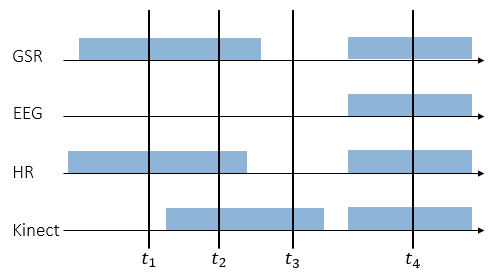
\includegraphics[width=0.75\columnwidth]{graphics/voting.png}
    \caption{The figure shows the different thresholds being satisfied for voting. $t_1$ depict the situation where two sensors agree, $t_2$ depict three, $t_3$ depict one and $t_4$ depict for all four}
    \label{[FIGURE] voting}
\end{figure}
\newcommand{\votinggraphs}[6]{
    \begin{figure}[h!]
    \begin{minipage}[t]{0.5\textwidth}
        \includegraphics[width=\linewidth,keepaspectratio=true]{graphics/graphs/voting/#1}
        \caption{#2}
        \label{#3}
    \end{minipage}
    \hspace*{\fill} % it's important not to leave blank lines before and after this command
    \begin{minipage}[t]{0.5\textwidth}
        \includegraphics[width=\linewidth,keepaspectratio=true]{graphics/graphs/voting/#4}
        \caption{#5}
        \label{#6}
    \end{minipage}
    \end{figure}
}

\newcommand{\easyvotinggraphs}[5]{ %y_axis caption1 label1 caption2 label2
  \votinggraphs
  {voting-False_cover_rate_(FCR)-#1-Aggressive.pdf}{#2}{#3}
  {voting-False_cover_rate_(FCR)-#1-Conservative.pdf}{#4}{#5}
}


\easyvotinggraphs{Events_hit_rate_(EHR)}
{Showing voting based on an aggressive scoring function. The lightest blue shade is 1 vote, and the darkest is 4 votes. The two shades in between are voting 2 and 3.}{fig:voting_aggresive_ehr}
{Showing voting based on a conservative scoring function. The lightest blue shade is 1 vote, and the darkest is 4 votes. The two shades in between are voting 2 and 3.}{fig:voting_conservative_ehr}


%\easyvotinggraphs{Precision}
%{Showing voting based on an aggressive scoring function}{fig:voting_aggressive_pres}
%{Showing voting based on a conservative scoring funtion}{fig:voting_conservative_pres}
\begin{table}[h]
  \centering
  \textbf{Conservative Approach}\vspace{2pt}
  \begin{tabularx}{\columnwidth}{cXXc}
    \toprule
    \textbf{Votes} & \textbf{Precision} & \textbf{EHR} & \textbf{FCR} \\
    \midrule
    1 & 40.0\% & 54.0\% & 42.8\% \\ \hline
    2 & 40.7\% & 23.2\% & 12.7\% \\ \hline
    3 & 33.6\% & 5.8\% & 1.9\% \\ \hline
    4 & 4.3\% & 0.5\% & 0.1\% \\ \hline
    \bottomrule
  \end{tabularx}

  \vspace{4pt}

  \textbf{Aggressive Approach}\vspace{2pt}
  \begin{tabularx}{\columnwidth}{cXXc}
    \toprule
    \textbf{Votes} & \textbf{Precision} & \textbf{EHR} & \textbf{FCR} \\
    \midrule
    1 & 37.6\% & 98.8\% & 91.9\% \\ \hline
    2 & 39.2\% & 92.2\% & 78.7\% \\ \hline
    3 & 41.4\% & 72.1\% & 58.0\% \\ \hline
    4 & 35.4\% & 33.7\% & 25.3\% \\ \hline
    \bottomrule
  \end{tabularx}

  \caption{Average statistics for voting}
  \label{[TABLE] avg_stats_voting}
\end{table}

As seen in Figure~\ref{fig:voting_aggresive_ehr}, the results from the aggressive approach for threshold 2 and 3 yielded reasonable results.
Voting 2 achieved 92.2\% EHR while having 79\% FCR data wrongly and 3 had 74.9\% EHR and 60.5\% FCR.
The result on threshold 2 are better than EEG which only achieved approximately 85\% EHR in the 80\% FCR range, and it
also performed better than the Kinect and EEG for threshold 3, however it did not show any improvements from the GSR and
HR results.
An average of the results can also be seen in Table~\ref{[TABLE] avg_stats_voting}

The conservative approach showed good tendencies at threshold 2 with 21.8\% EHR and 12.3\% FCR, as seen in Figure~\ref{fig:voting_conservative_ehr}.
Results are better than the EEG and Kinect in the conservative aspect, however it does not seem to gain any significant advantages compared to the HR and GSR.
As expected, the results from threshold 3 and 4 revealed little to no points of interest, and threshold 1 showed a bad EHR to FCR ratio. 
The results from the conservative approach can also be seen in Table~\ref{[TABLE] avg_stats_voting}.

Both approaches showed improvements compared to EEG and Kinect, but it did not give any decidedly results for good or worse compared
to HR and GSR.
Even though voting did not yield any better results than HR and GSR, it seem to have opted the stability across the four sensors. If this were to be used in a real usability test voting could potentially be used to keep the stability of the result at a reasonable level. 
